\documentclass[a4paper]{article}
\usepackage{mathtools,amssymb,amsthm}
\usepackage[top=2.5cm,bottom=2.5cm,right=2.5cm,left=2.5cm]{geometry}
\usepackage{tikz}
\usetikzlibrary{positioning}
\usepackage{algorithm}
\usepackage{algpseudocode}


\title{Fully connected NN}
\author{Remi Chassagnol}
\date{\today}

\begin{document}

\newcommand{\ajl}{a_{j}^{l}}
\newcommand{\ajll}{a_{j}^{l-1}}
\newcommand{\akll}{a_{k}^{l-1}}
\newcommand{\ajL}{a_{j}^{L}}
\newcommand{\akL}{a_{k}^{L}}
\newcommand{\aL}{a^{L}}

\newcommand{\zjl}{z_{j}^{l}}
\newcommand{\zjll}{z_{j}^{l-1}}
\newcommand{\zl}{z^{l}}
\newcommand{\zlp}{z^{l+1}}
\newcommand{\zklp}{z_{k}^{l+1}}
\newcommand{\zjL}{z_{j}^{L}}
\newcommand{\zkL}{z_{k}^{L}}
\newcommand{\zL}{z^{L}}

\newcommand{\wjkl}{w_{jk}^{l}}
\newcommand{\wjkll}{w_{jk}^{l-1}}
\newcommand{\wjklp}{w_{jk}^{l+1}}
\newcommand{\wlp}{w^{l+1}}

\newcommand{\bjl}{b_{j}^{l}}
\newcommand{\bjll}{b_{j}^{l-1}}

\newcommand{\errjl}{\delta_{j}^{l}}
\newcommand{\errjll}{\delta_{j}^{l-1}}
\newcommand{\errl}{\delta^{l}}
\newcommand{\errlp}{\delta^{l+1}}
\newcommand{\errklp}{\delta_{k}^{l+1}}
\newcommand{\errjL}{\delta_{j}^{L}}
\newcommand{\errL}{\delta^{L}}
  
\maketitle

\section{Notations}

\begin{itemize}
  \item $\wjkl$ is the weight of the $k^{th}$ neuron in the layer $(l - 1)$
    to the $j^{th}$ neuron in the layer $l$
  \item $\bjl$ is the bias of the $j^{th}$ neuron on the layer $l$.
  \item $\ajl$ is the activation of the $j^{th}$ neuron on the layer $l$.
  \item $act$ is the activation function.
  \item $cost$ is the cost function.
  \item $\errjl$ is the error of the $j^{th}$ neuron on the layer $l$.
  \item $L$ is the last layer.
\end{itemize}

\begin{center}
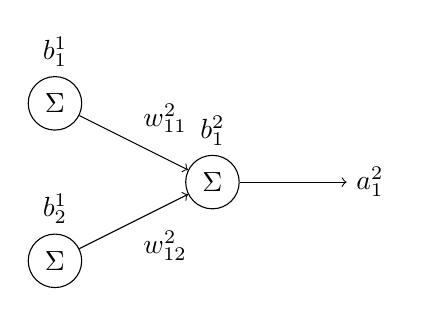
\begin{tikzpicture}
  % \draw[step=0.5cm,gray,very thin] (0,0) grid (6,6);
  %Nodes
  \node at (0,2) [circle,draw=black,label=$b_{1}^{1}$] (prevneuron1) {$\Sigma$};
  \node at (0,0) [circle,draw=black,label=$b_{2}^{1}$] (prevneuron2) {$\Sigma$};
  \node at (2,1) [circle,draw=black,label=$b_{1}^{2}$] (neuron) {$\Sigma$};
  \node at (4,1) (result) {$a_{1}^{2}$};

  %Lines
  \draw[->] (prevneuron1) to node [auto] {$w_{11}^{2}$} (neuron);
  \draw[->] (prevneuron2) to node [auto,swap] {$w_{12}^{2}$} (neuron);
  \draw[->] (neuron) to (result);
\end{tikzpicture}
\end{center}


\clearpage{}
\section{Definitions}

Transition from the layer $(l - 1)$ to the layer $l$:

\begin{align}
  \zjl &= \sum_{k}{\wjkl\akll + \bjl} \\
  \ajl &= act(\zjl)
\end{align}

The error of a neuron can be define as:

\begin{align}
  \errjl \equiv \frac{\partial cost}{\partial \zjl}
\end{align}

We define $\errjL$ the error on the output layer as the following:

\begin{align}
  \errjL = \frac{\partial cost}{\partial \ajl}act'(\zjL)
\end{align}

Then we have $\errL$ which is a vector that contains the errors of all the
output neurons:

\begin{align}
  \errL &= \nabla_{a} cost \odot act'(\zL)
\end{align}

Here, we can deduce the value of $\errl$:

\begin{align}
  \errl &= ((\wlp)^{T}\errlp) \odot act'(\zl)
\end{align}

Now that we have this, we can define the error in terms of $w$ and $b$:

\begin{align}
  \frac{\partial cost}{\partial \bjl} &= \errjl \\
  \frac{\partial cost}{\partial \wjkl} &= \akll \errjl
\end{align}


\clearpage{}
\section{Algorithms}

First we wan to apply the model to the input by making the data flow threw the
network using the feed forward algorithm.

\begin{algorithm}
  \caption{FeedForward}
  \begin{algorithmic}
    \Procedure{FeedForward}{$weights$, $biases$, $input$}
      \State $a$ = $input$
      \State $as$ = [$a$]
      \State $zs$ = []\\

      \For{$w$, $b$ in ($weights$, $biases$)}
          \State $z = w \times a + b$
          \State append($zs$, $z$)
          \State $a$ = act($z$)
          \State append($as$, $a$)
      \EndFor
      \State \textbf{return} $as$, $zs$
    \EndProcedure
  \end{algorithmic}
\end{algorithm}

Then we compute the gradiant of all the nodes using the back propagation
(propagate the result error back in the network).

\begin{algorithm}
  \caption{Back propagation algorithm}
  \begin{algorithmic}
    \Procedure{BackPropagate}{$as$, $zs$, $weights$, $biases$}
      \State $deltas$ = cost'($as[L - 1]$, $expected\_solution$) $\odot$ act'($zs[L - 1]$)
      \State $grads\_b[L - 1]$ = $deltas$
      \State $grads\_w[L - 1]$ = matmul($deltas$, act'($a[L - 2]$)) \\

      \For{$l$ in $(L - 2)$..=0}
        \State $deltas$ = matmul($weights[l + 1]$, $deltas$) $\odot$ act'($zs[l]$)
        \State $grads\_b[l]$ = $deltas$
        \State $grads\_w[l]$ = matmul($deltas$, act'($a[l - 1]$))
      \EndFor

      \State \textbf{return} $grads\_w$, $grads\_b$
    \EndProcedure
  \end{algorithmic}
\end{algorithm}

The last component we need is the optimize function that will update the weights
and the biases. There are various ways to do this, here is an example for a
stochastic gradiant descant:

\begin{algorithm}
  \caption{Optimization for a stochastic gradiant descant}
  \begin{algorithmic}
    \Procedure{Optimize}{$weights$, $biases$, $grads\_w$, $grads\_b$, $l\_rate$}
      \For{$l$ in 0..<L}
        \State $weights[l]$ -= $l\_rate \times grads\_w[l]$
        \State $biases[l]$ -= $l\_rate \times grads\_b[l]$
      \EndFor

      \State \textbf{return} $weights$, $biases$
    \EndProcedure
  \end{algorithmic}
\end{algorithm}

To train, we usually use minibatches. This means that we compute the average
error on all the minibatches before updating the weights and biases.

\begin{algorithm}
  \caption{Update the weights using a minibatch}
  \begin{algorithmic}
    \Procedure{UpdateMinibatch}{$weights$, $biases$, $minibatches$, $l\_rate$}
      \State $grads\_w\_total$ = $0$
      \State $grads\_b\_total$ = $0$ \\

      \For{$minibatch$ in $minibatches$}
        \State $as$, $zs$ = FeedForward($weights$, $biases$, $minibatch$)
        \State $grads\_w$, $grads\_b$ = BackPropagate($as$, $zs$, $weights$, $biases$)
        \State $grads\_w\_total$ += $grads\_w$
        \State $grads\_b\_total$ += $grads\_b$
      \EndFor
      \State $grads\_w$ = $grads\_w\_total$ / size($minibatches$)
      \State $grads\_b$ = $grads\_b\_total$ / size($minibatches$)
      \State $weights$, $biases$ = Optimize($weights$, $biases$, $grads\_w$, $grads\_b$, $l\_rate$) \\

      \State \textbf{return} $weights$, $biases$
    \EndProcedure
  \end{algorithmic}
\end{algorithm}

\clearpage
\section{Proofs}

\subsubsection{Error on the output layer $\errjL$}

Let's prove the following:

\begin{align}
  \errjL &= \frac{\partial cost}{\partial \ajL}act'(\zjL) \\
         &= \frac{\partial cost}{\partial \ajL} \frac{\partial act}{\partial \zjL}
\end{align}

The definition of the error is:

\begin{align}
  \errjL &= \frac{\partial cost}{\partial \zjL} \\
         &= \sum_{k}{\frac{\partial cost}{\partial \akL} \frac{\partial \akL}{\partial \zjL}}
\end{align}

Since $\akL = act(\zkL)$, if $j \neq k$, then $\frac{\partial \akL}{\partial \zjL} = 0$.
Which gives the result expression:

\begin{align}
  \errjL = \frac{\partial cost}{\partial \ajL} \frac{\partial \ajL}{\partial \zjL}
\end{align}

\subsubsection{Error on internal layers $\errjl$}

$\errjl$ is defined as:

\begin{align}
  \errjl &= \frac{\partial cost}{\partial \zjl} \\
         &= \sum_{k}{\frac{\partial cost}{\partial \zklp}\frac{\partial \zklp}{\partial \zjl}} \\
         &= \sum_{k}{\errklp\frac{\partial \zklp}{\partial \zjl}}
\end{align}

We can then define $\zklp$ as:

\begin{align}
  \zklp = \sum_{j}{w_{kj}^{l+1}act(z_{j}^{l}) + b_{k}^{l+1}}
\end{align}

so the derivative is:

\begin{align}
  \frac{\zklp}{\zjl} = w_{kj}^{l+1}act'(z_{j}^{l})
\end{align}

Substituing back to the original formula:

\begin{align}
  \errjl &= \sum_{k}{w_{kj}^{l+1} \errklp act'(z_{j}^{l})}
\end{align}

\subsubsection{Bias gradiant $\frac{\partial cost}{\partial \bjl}$}

We prove the following:

\begin{align}
  \frac{\partial cost}{\partial \bjl} = \errjl
\end{align}

We can rewrite it like the following:

\begin{align}
  \frac{\partial cost}{\partial \bjl} = 
    \sum_{k}{
      \frac{\partial cost}{\partial \zklp}
      \frac{\partial \zklp}{\partial \zjl}
      \frac{\partial \zjl}{\partial \bjl}
    }
\end{align}

since $\frac{\partial \zjl}{\partial \bjl} = 1$, then:

\begin{align}
  \frac{\partial cost}{\partial \bjl} &= 
    \sum_{k}{
      \frac{\partial cost}{\partial \zklp}
      \frac{\partial \zklp}{\partial \zjl}
    } \\
    &= \errjl
\end{align}

\subsubsection{Bias gradiant $\frac{\partial cost}{\partial \wjkl}$}

We prove the following:

\begin{align}
  \frac{\partial cost}{\partial \wjkl} = \akll \errjl
\end{align}

We can rewrite it like the following:

\begin{align}
  \frac{\partial cost}{\partial \wjkl} = 
    \sum_{k}{
      \frac{\partial cost}{\partial \zklp}
      \frac{\partial \zklp}{\partial \zjl}
      \frac{\partial \zjl}{\partial \wjkl}
    }
\end{align}

since $\frac{\partial \zjl}{\partial \wjkl} = \akll$, then:

\begin{align}
  \frac{\partial cost}{\partial \wjkl} &= 
    \sum_{k}{
      \frac{\partial cost}{\partial \zklp}
      \frac{\partial \zklp}{\partial \zjl}
      \akll
    } \\
    &= \errjl \akll
\end{align}

\end{document}
